% The original template (from Trevor) had a custom \appendix command,
% but I found it to break figure/table counters. I'm not sure how
% reliable my fix is, so I ended up reverting back to the standard
% latex version, and renaming the custom command to \myappendix.  You
% can try both and see how things work out:
% 1) Call \appendix once, and then make each appendix a \chapter
% 2) Call \myappendix once, and then make each appendix a \section.

\appendix
\chapter{Supplementary figures}
\begin{figure}[htp]
		\centering
	    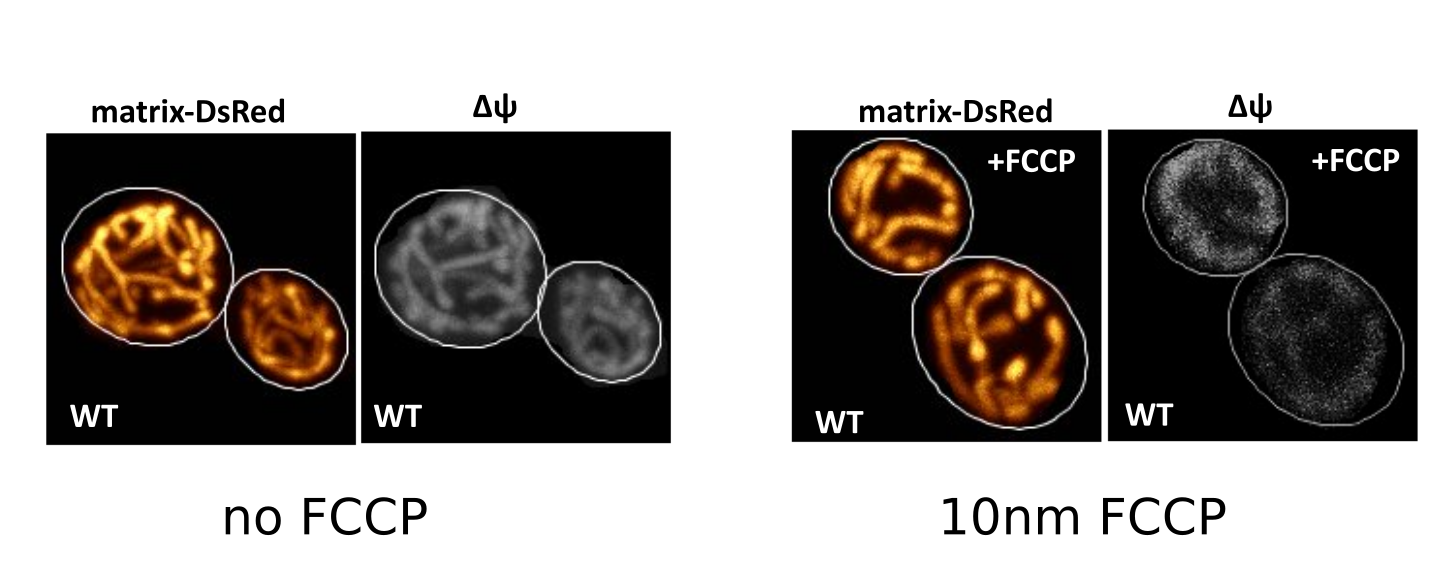
\includegraphics[width=\textwidth]{fccp}
	    \caption{Shown in this figure are images of cells stained with 100nm of DiOC$_6$, a membrane potential dependent dye (ΔΨ). The image on the left is a cell that is undergoing respiration and has normal levels of ΔΨ. The image on the right is a cell that has been treated with an uncoupler of ΔΨ, FCCP. The ΔΨ of the mitochondria is almost completely abolished after treatment, indicating that the dye was not suffering from auto-quenching (i.e. DiOC$_6$ signal intensity was proportional to ΔΨ).\\[2ex]\emph{Image provided courtesy of V.Jayashankar.}}\label{fig:fccp}
\end{figure}
%
%
\begin{figure}[htp]
		\centering
	    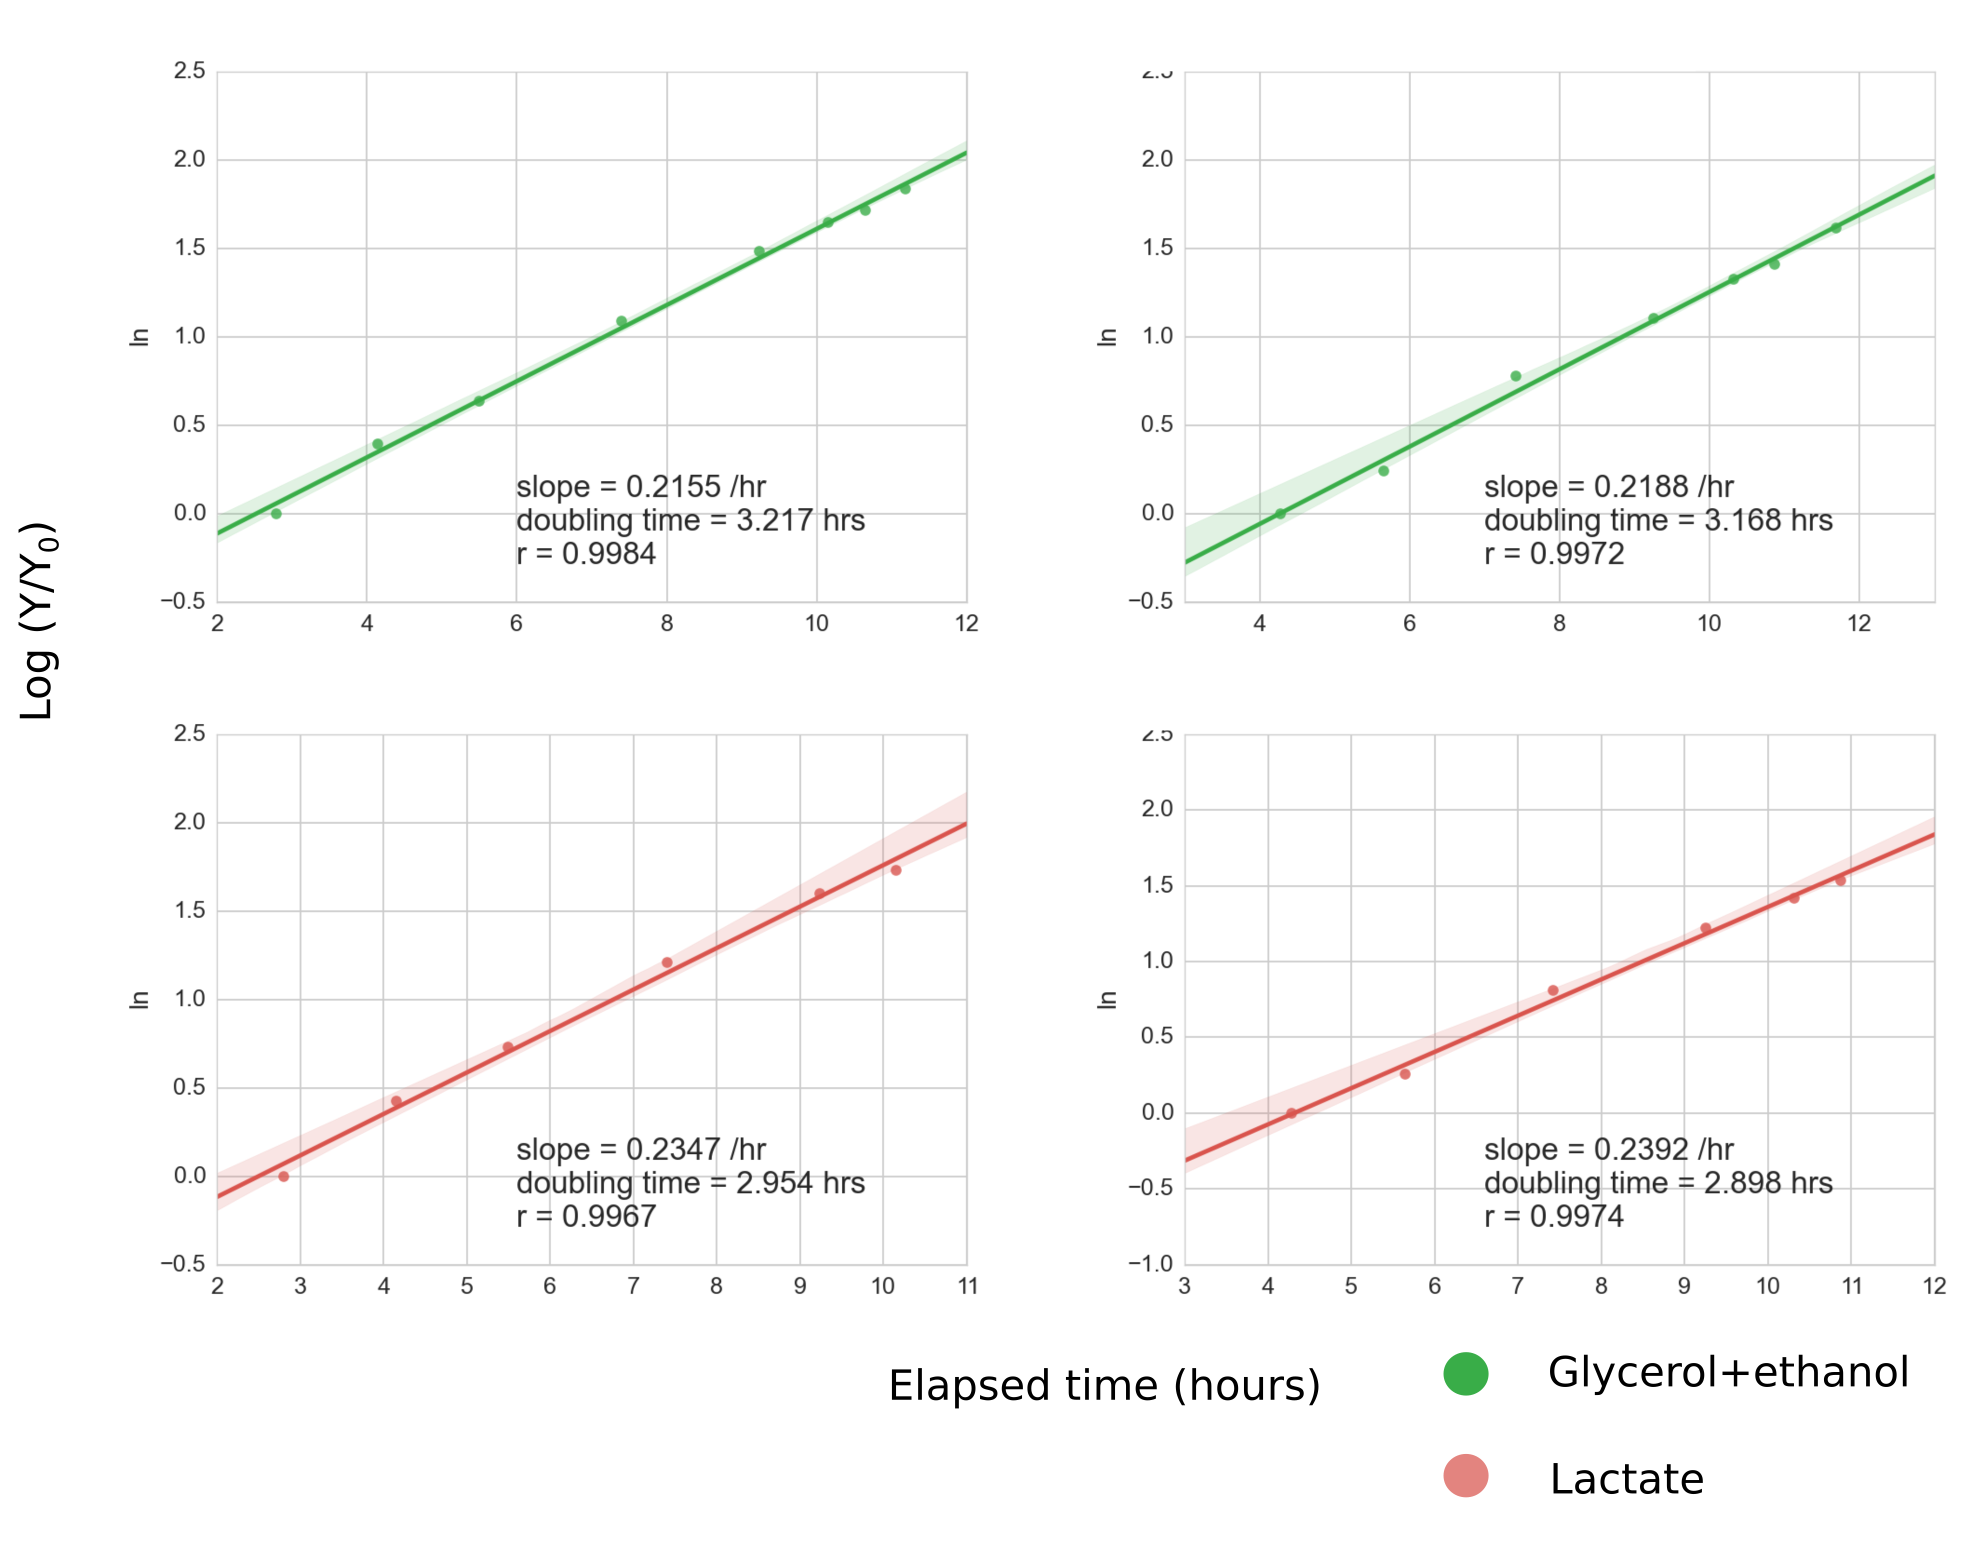
\includegraphics[width=\textwidth]{grwthcvs}
	    \caption{Shown in this figure are the growth curves for 2 replicates of yeast undergoing exponential growth in either YP+2\% glycerol+2\% ethanol or YP+2\% lactate. The doubling times for lactate was just slightly longer than glycerol+ethanol (3.2 hours vs 2.9 hours).}\label{fig:grwtcvs}
\end{figure}
%
%
\begin{figure}[htp]
		\centering
	    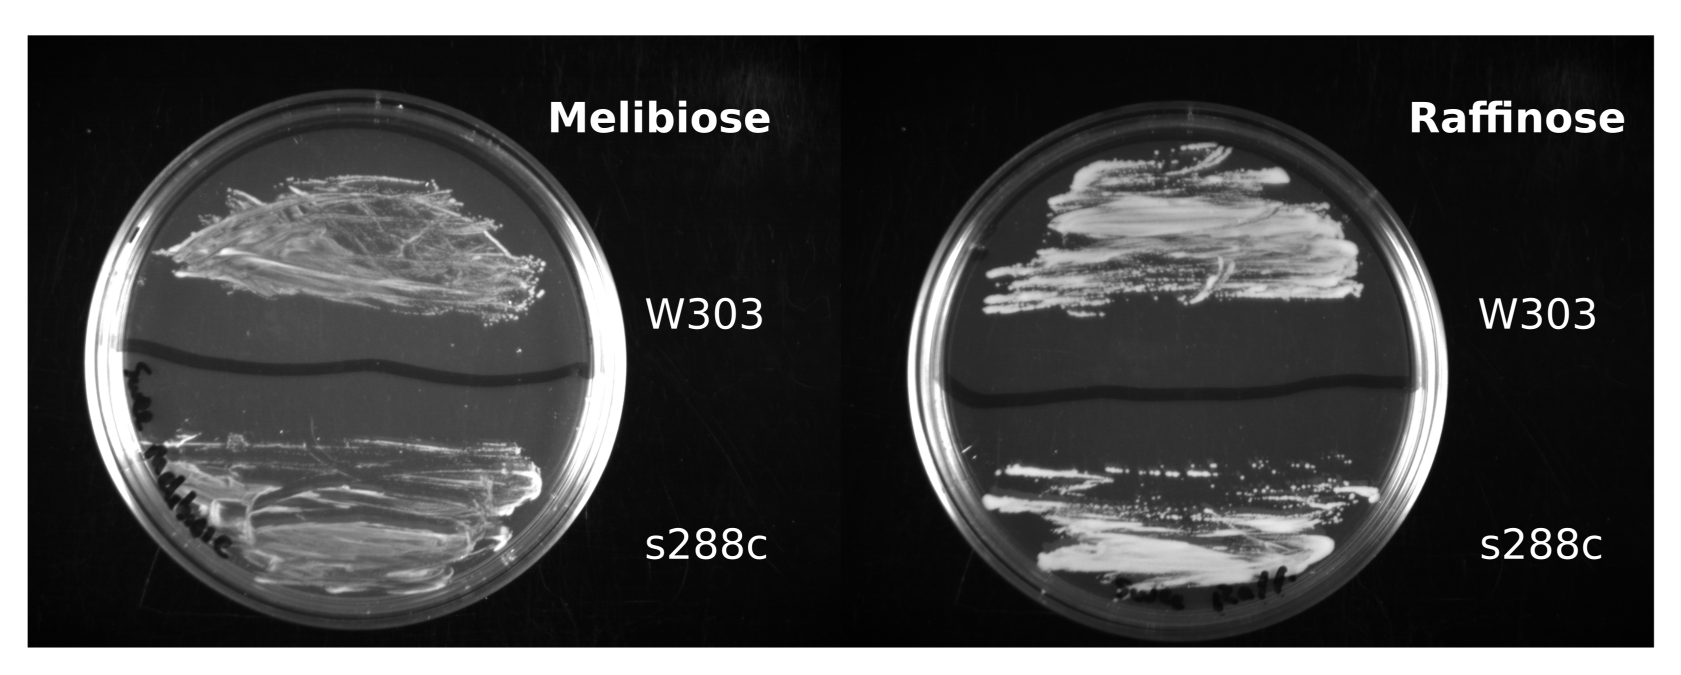
\includegraphics[width=\textwidth]{meli}
	    \caption{Shown in this figure are streak plates of W303a strain used in this thesis together with a s288c strain to check for growth viability on melibiose and raffinose. The plates were yeast extract+peptone+either 2\% melibiose or 2\% raffinose. Imaging of the plates was taken 4 days after streaking.}\label{fig:meli}
\end{figure}
%
%	    
\chapter{Statistical tables}
%
{
\sisetup{
round-mode = places,
round-precision = 4}
\begin{table}
\caption{Tables of statistical tests using rank-sums test with Holms -Sidak post-hoc multiple testing correction.\\Labels---YPD = glucose, YPE = glycerol+ethanol, YPL = lactate, YPR = raffinose\\stat = rank sum statistic\\p-val = uncorrected rank sum $p$ value\\
pval-corr. = Holms-Sidak multiple testing correction $p$ value\\
Test criteria--- reject null hypothesis that there is no difference between the medians of the group if pval-corr < 0.05\\Values with 0.0000 indicate $p$ < 1×10$^{-27}$}\label{tab:tests}
\centering
\footnotesize
\begin{tabular}{x{2cm}x{2cm}S[round-mode = places,round-precision = 0,table-format=4.0]S[table-format=2.4]S[table-format=2.4]c}
\toprule
\multicolumn{2}{c}{\textbf{Cell mito avg. ΔΨ scl.}}&&&\\
\cmidrule{1-2}
\textbf{group1} & \textbf{group2} & \textbf{stat} &\textbf{p-val}&\textbf{p-val corr.}& \textbf{reject}  \\
\midrule
      YPD       &       YPE       &     5052.0    &     0.2607    &       0.5661       &      False       \\
      YPD       &       YPL       &     4605.0    &     0.0120     &       0.0619       &      False       \\
      YPD       &       YPR       &     4579.0    &     0.4705    &       0.5661       &      False       \\
      YPE       &       YPL       &     5592.0    &     0.0352    &       0.1334       &      False       \\
      YPE       &       YPR       &     5028.0    &     0.2429    &       0.5661       &      False       \\
      YPL       &       YPR       &     4584.0    &     0.0106    &       0.0619       &      False       \\
\bottomrule
\end{tabular}
\end{table}
%
\begin{table}
\centering
\footnotesize
\begin{tabular}{x{2cm}x{2cm}S[round-mode = places,round-precision = 0,table-format=4.0]S[table-format=2.4]S[table-format=2.4]c}
\toprule
\multicolumn{2}{c}{\textbf{Cell mito avg. ΔΨ raw}}&&&\\
\cmidrule{1-2}
\textbf{group1} & \textbf{group2} & \textbf{stat} &\textbf{p-val}&\textbf{p-val corr.}& \textbf{reject}  \\
\midrule
      YPD       &       YPE       &     629.0     &      0.0      &        0.0         &       True       \\
      YPD       &       YPL       &     1402.0    &      0.0      &        0.0         &       True       \\
      YPD       &       YPR       &     939.0     &      0.0      &        0.0         &       True       \\
      YPE       &       YPL       &     4198.0    &      0.0      &        0.0         &       True       \\
      YPE       &       YPR       &     4085.0    &     0.0019    &       0.0038       &       True       \\
      YPL       &       YPR       &     4985.0    &     0.0795    &       0.0795       &      False       \\
\bottomrule
\end{tabular}
\end{table}
%
\begin{table}
\centering
\footnotesize
\begin{tabular}{x{2cm}x{2cm}S[round-mode = places,round-precision = 0,table-format=4.0]S[table-format=2.4]S[table-format=2.4]c}
\toprule
\multicolumn{2}{c}{\textbf{Cell mito std. ΔΨ scl.}}&&&\\
\cmidrule{1-2}
\textbf{group1} & \textbf{group2} & \textbf{stat} &\textbf{p-val}&\textbf{p-val corr.}& \textbf{reject}  \\
\midrule
      YPD       &       YPE       &     5050.0    &     0.2592    &       0.6337       &      False       \\
      YPD       &       YPL       &     5273.0    &     0.2221    &       0.6337       &      False       \\
      YPD       &       YPR       &     4368.0    &     0.2669    &       0.6337       &      False       \\
      YPE       &       YPL       &     5697.0    &     0.0549    &       0.2874       &      False       \\
      YPE       &       YPR       &     4728.0    &     0.0815    &       0.3463       &      False       \\
      YPL       &       YPR       &     5606.0    &     0.4915    &       0.6337       &      False       \\
\bottomrule
\end{tabular}
\end{table}

%
\begin{table}
\centering
\footnotesize
\begin{tabular}{x{2cm}x{2cm}S[round-mode = places,round-precision = 0,table-format=4.0]S[table-format=2.4]S[table-format=2.4]c}
\toprule
\multicolumn{2}{c}{\textbf{Cell mito std. ΔΨ raw}}&&&\\
\cmidrule{1-2}
\textbf{group1} & \textbf{group2} & \textbf{stat} &\textbf{p-val}&\textbf{p-val corr.}& \textbf{reject}  \\
\midrule
      YPD       &       YPE       &     1060.0    &      0.0      &        0.0         &       True       \\
      YPD       &       YPL       &     2201.0    &      0.0      &        0.0         &       True       \\
      YPD       &       YPR       &     1398.0    &      0.0      &        0.0         &       True       \\
      YPE       &       YPL       &     4205.0    &      0.0      &        0.0         &       True       \\
      YPE       &       YPR       &     4219.0    &     0.005     &       0.0099       &       True       \\
      YPL       &       YPR       &     4860.0    &     0.0457    &       0.0457       &       True       \\
\bottomrule
\end{tabular}
\end{table}
%
\begin{table}
\centering
\footnotesize
\begin{tabular}{x{2cm}x{2cm}S[round-mode = places,round-precision = 0,table-format=4.0]S[table-format=2.4]S[table-format=2.4]c}
\toprule
\multicolumn{2}{c}{\textbf{Network avg. deg.}}&&&\\
\cmidrule{1-2}
\textbf{group1} & \textbf{group2} & \textbf{stat} &\textbf{p-val}&\textbf{p-val corr.}& \textbf{reject}  \\
\midrule
      YPD       &       YPE       &     3685.0    &     0.0001    &       0.0003       &       True       \\
      YPD       &       YPL       &     3331.0    &      0.0000      &        0.0         &       True       \\
      YPD       &       YPR       &     3279.5    &     0.0003    &       0.0011       &       True       \\
      YPE       &       YPL       &     5791.5    &     0.0794    &       0.2198     &      False       \\
      YPE       &       YPR       &     5280.5    &     0.4564    &       0.4564       &      False       \\
      YPL       &       YPR       &     4999.0    &     0.0842    &       0.2198       &      False       \\
\bottomrule
\end{tabular}
\end{table}
%
\begin{table}
\centering
\footnotesize
\begin{tabular}{x{2cm}x{2cm}S[round-mode = places,round-precision = 0,table-format=4.0]S[table-format=2.4]S[table-format=2.4]c}
\toprule
\multicolumn{2}{c}{\textbf{Shortest path len.}}&&&\\
\cmidrule{1-2}
\textbf{group1} & \textbf{group2} & \textbf{stat} &\textbf{p-val}&\textbf{p-val corr.}& \textbf{reject}  \\
\midrule
      YPD       &       YPE       &     3292.0    &      0.0      &        0.0         &       True       \\
      YPD       &       YPL       &     808.5     &      0.0      &        0.0         &       True       \\
      YPD       &       YPR       &     2716.0    &      0.0      &        0.0         &       True       \\
      YPE       &       YPL       &     2256.0    &      0.0      &        0.0         &       True       \\
      YPE       &       YPR       &     5138.0    &     0.3296    &       0.3296       &      False       \\
      YPL       &       YPR       &     2140.5    &      0.0      &        0.0         &       True       \\
\bottomrule
\end{tabular}
\end{table}
%
\begin{table}
\centering
\footnotesize
\begin{tabular}{x{2cm}x{2cm}S[round-mode = places,round-precision = 0,table-format=4.0]S[table-format=2.4]S[table-format=2.4]c}
\toprule
\multicolumn{2}{c}{\textbf{Number of edges}}&&&\\
\cmidrule{1-2}
\textbf{group1} & \textbf{group2} & \textbf{stat} &\textbf{p-val}&\textbf{p-val corr.}& \textbf{reject}  \\
\midrule
      YPD       &       YPE       &     2996.0    &      0.0      &        0.0         &       True       \\
      YPD       &       YPL       &     524.0     &      0.0      &        0.0         &       True       \\
      YPD       &       YPR       &     2804.5    &      0.0      &        0.0         &       True       \\
      YPE       &       YPL       &     1933.0    &      0.0      &        0.0         &       True       \\
      YPE       &       YPR       &     5142.0    &     0.3329    &       0.3329       &      False       \\
      YPL       &       YPR       &     1461.0    &      0.0      &        0.0         &       True       \\
\bottomrule
\end{tabular}
\end{table}
%
\begin{table}
\centering
\footnotesize
\begin{tabular}{x{2cm}x{2cm}S[round-mode = places,round-precision = 0,table-format=4.0]S[table-format=2.4]S[table-format=2.4]c}
\toprule
\multicolumn{2}{c}{\textbf{Cell $\text{β}_{\V{geometric}}$}}&&&\\
\cmidrule{1-2}
\textbf{group1} & \textbf{group2} & \textbf{stat} &\textbf{p-val}&\textbf{p-val corr.}& \textbf{reject}  \\
\midrule
      YPD       &       YPE       &     3882.5    &     0.0004    &       0.0015       &       True       \\
      YPD       &       YPL       &     3695.5    &      0.0      &       0.0001       &       True       \\
      YPD       &       YPR       &     3121.0    &     0.0001    &       0.0003       &       True       \\
      YPE       &       YPL       &     6186.5    &     0.269     &       0.5672       &      False       \\
      YPE       &       YPR       &     5029.0    &     0.2436    &       0.5672       &      False       \\
      YPL       &       YPR       &     5585.5    &     0.4733    &       0.5672       &      False       \\
\bottomrule
\end{tabular}
\end{table}
%
\begin{table}
\centering
\footnotesize
\begin{tabular}{x{2cm}x{2cm}S[round-mode = places,round-precision = 0,table-format=4.0]S[table-format=2.4]S[table-format=2.4]c}
\toprule
\multicolumn{2}{c}{\textbf{Cell $\text{β}_{\V{topological}}$}}&&&\\
\cmidrule{1-2}
\textbf{group1} & \textbf{group2} & \textbf{stat} &\textbf{p-val}&\textbf{p-val corr.}& \textbf{reject}  \\
\midrule
      YPD       &       YPE       &     3982.0    &     0.0009    &       0.0034       &       True       \\
      YPD       &       YPL       &     3793.0    &      0.0      &       0.0001       &       True       \\
      YPD       &       YPR       &     3180.5    &     0.0001    &       0.0005       &       True       \\
      YPE       &       YPL       &     6030.5    &     0.1762    &       0.4408       &      False       \\
      YPE       &       YPR       &     5030.5    &     0.2444    &       0.4408       &      False       \\
      YPL       &       YPR       &     5515.0    &     0.4111    &       0.4408       &      False       \\
\bottomrule
\end{tabular}
\end{table}
%
\begin{table}
\centering
\footnotesize
\begin{tabular}{x{2cm}x{2cm}S[round-mode = places,round-precision = 0,table-format=4.0]S[table-format=2.4]S[table-format=2.4]c}
\toprule
\multicolumn{2}{c}{\textbf{Cell φ}}&&&\\
\cmidrule{1-2}
\textbf{group1} & \textbf{group2} & \textbf{stat} &\textbf{p-val}&\textbf{p-val corr.}& \textbf{reject}  \\
\midrule
      YPD       &       YPE       &     3928.5    &     0.0006    &       0.0022       &       True       \\
      YPD       &       YPL       &     3785.5    &      0.0      &       0.0001       &       True       \\
      YPD       &       YPR       &     3113.0    &     0.0001    &       0.0003       &       True       \\
      YPE       &       YPL       &     6028.5    &     0.1751    &       0.4387       &      False       \\
      YPE       &       YPR       &     5000.5    &     0.2229    &       0.4387       &      False       \\
      YPL       &       YPR       &     5524.5    &     0.4193    &       0.4387       &      False       \\
\bottomrule
\end{tabular}
\end{table}
%
\begin{table}
\centering
\footnotesize
\begin{tabular}{x{2cm}x{2cm}S[round-mode = places,round-precision = 0,table-format=4.0]S[table-format=2.4]S[table-format=2.4]c}
\toprule
\multicolumn{2}{c}{\textbf{Cell Pk$_3$}}&&&\\
\cmidrule{1-2}
\textbf{group1} & \textbf{group2} & \textbf{stat} &\textbf{p-val}&\textbf{p-val corr.}& \textbf{reject}  \\
\midrule
      YPD       &       YPE       &     3759.0    &     0.0001    &       0.0007       &       True       \\
      YPD       &       YPL       &     3475.5    &      0.0      &        0.0         &       True       \\
      YPD       &       YPR       &     3222.0    &     0.0002    &       0.0007       &       True       \\
      YPE       &       YPL       &     5815.5    &     0.0868    &       0.2384       &      False       \\
      YPE       &       YPR       &     5168.5    &     0.3557    &       0.4005       &      False       \\
      YPL       &       YPR       &     5278.5    &     0.2257    &       0.4005       &      False       \\
\bottomrule
\end{tabular}
\end{table}
%
\begin{table}
\centering
\footnotesize
\begin{tabular}{x{2cm}x{2cm}S[round-mode = places,round-precision = 0,table-format=4.0]S[table-format=2.4]S[table-format=2.4]c}
\toprule
\multicolumn{2}{c}{\textbf{Total network length}}&&&\\
\cmidrule{1-2}
\textbf{group1} & \textbf{group2} & \textbf{stat} &\textbf{p-val}&\textbf{p-val corr.}& \textbf{reject}  \\
\midrule
      YPD       &       YPE       &     2221.0    &      0.0      &        0.0         &       True       \\
      YPD       &       YPL       &     321.0     &      0.0      &        0.0         &       True       \\
      YPD       &       YPR       &     2234.0    &      0.0      &        0.0         &       True       \\
      YPE       &       YPL       &     2204.0    &      0.0      &        0.0         &       True       \\
      YPE       &       YPR       &     4936.0    &     0.1812    &       0.1812       &      False       \\
      YPL       &       YPR       &     1585.0    &      0.0      &        0.0         &       True       \\
\bottomrule
\end{tabular}
\end{table}
%
\begin{table}
\centering
\footnotesize
\begin{tabular}{x{2cm}x{2cm}S[round-mode = places,round-precision = 0,table-format=4.0]S[table-format=2.4]S[table-format=2.4]c}
\toprule
\multicolumn{2}{c}{\textbf{$\frac{\text{shortest path length}}{\text{total length}}$}}&&&\\
\cmidrule{1-2}
\textbf{group1} & \textbf{group2} & \textbf{stat} &\textbf{p-val}&\textbf{p-val corr.}& \textbf{reject}  \\
\midrule
      YPD       &       YPE       &     3713.0    &     0.0001    &       0.0003       &       True       \\
      YPD       &       YPL       &     2867.0    &      0.0      &        0.0         &       True       \\
      YPD       &       YPR       &     3733.0    &     0.0116    &       0.023        &       True       \\
      YPE       &       YPL       &     5094.0    &     0.0025    &       0.0074       &       True       \\
      YPE       &       YPR       &     4608.0    &     0.0471    &       0.0471       &       True       \\
      YPL       &       YPR       &     3634.0    &      0.0      &        0.0         &       True       \\
\bottomrule
\end{tabular}
\end{table}
%
\begin{table}
\centering
\footnotesize
\begin{tabular}{x{2cm}x{2cm}S[round-mode = places,round-precision = 0,table-format=4.0]S[table-format=2.4]S[table-format=2.4]c}
\toprule
\multicolumn{2}{c}{\textbf{$\frac{\text{shortest path length}}{\text{Num. of edges}}$}}&&&\\
\cmidrule{1-2}
\textbf{group1} & \textbf{group2} & \textbf{stat} &\textbf{p-val}&\textbf{p-val corr.}& \textbf{reject}  \\
\midrule
      YPD       &       YPE       &     4257.0    &     0.0064    &       0.019        &       True       \\
      YPD       &       YPL       &     2202.0    &      0.0      &        0.0         &       True       \\
      YPD       &       YPR       &     4038.0    &     0.0695    &       0.1342       &      False       \\
      YPE       &       YPL       &     3175.0    &      0.0      &        0.0         &       True       \\
      YPE       &       YPR       &     4959.0    &     0.1956    &       0.1956       &      False       \\
      YPL       &       YPR       &     2404.0    &      0.0      &        0.0         &       True       \\
\bottomrule
\end{tabular}
\end{table}
%
\begin{table}
\centering
\footnotesize
\begin{tabular}{x{2cm}x{2cm}S[round-mode = places,round-precision = 0,table-format=4.0]S[table-format=2.4]S[table-format=2.4]c}
\toprule
\multicolumn{2}{c}{\textbf{Cell coef.var. ΔΨ scl.}}&&&\\
\cmidrule{1-2}
\textbf{group1} & \textbf{group2} & \textbf{stat} &\textbf{p-val}&\textbf{p-val corr.}& \textbf{reject}  \\
\midrule
      YPD       &       YPE       &     5199.0    &     0.3825    &       0.7645       &      False       \\
      YPD       &       YPL       &     4822.0    &     0.0381    &       0.144        &      False       \\
      YPD       &       YPR       &     4597.0    &     0.4891    &       0.7645       &      False       \\
      YPE       &       YPL       &     5130.0    &     0.0031    &       0.0184       &       True       \\
      YPE       &       YPR       &     5205.0    &     0.3878    &       0.7645       &      False       \\
      YPL       &       YPR       &     4699.0    &     0.0203    &       0.0974       &      False       \\
\bottomrule
\end{tabular}
\end{table}
%
\begin{table}
\centering
\footnotesize
\begin{tabular}{x{2cm}x{2cm}S[round-mode = places,round-precision = 0,table-format=4.0]S[table-format=2.4]S[table-format=2.4]c}
\toprule
\multicolumn{2}{c}{\textbf{Cell coef.var. ΔΨ raw}}&&&\\
\cmidrule{1-2}
\textbf{group1} & \textbf{group2} & \textbf{stat} &\textbf{p-val}&\textbf{p-val corr.}& \textbf{reject}  \\
\midrule
      YPD       &       YPE       &     1650.0    &      0.0      &        0.0         &       True       \\
      YPD       &       YPL       &     1870.0    &      0.0      &        0.0         &       True       \\
      YPD       &       YPR       &     1781.0    &      0.0      &        0.0         &       True       \\
      YPE       &       YPL       &     5628.0    &     0.0411    &       0.1184       &      False       \\
      YPE       &       YPR       &     4623.0    &     0.0506    &       0.1184       &      False       \\
      YPL       &       YPR       &     5527.0    &     0.4216    &       0.4216       &      False       \\
\bottomrule
\end{tabular}
\end{table}
%
\begin{table}
\centering
\footnotesize
\begin{tabular}{x{2cm}x{2cm}S[round-mode = places,round-precision = 0,table-format=4.0]S[table-format=2.4]S[table-format=2.4]c}
\toprule
\multicolumn{2}{c}{\textbf{Cell GFP intensity}}&&&\\
\cmidrule{1-2}
\textbf{group1} & \textbf{group2} & \textbf{stat} &\textbf{p-val}&\textbf{p-val corr.}& \textbf{reject}  \\
\midrule
      YPD       &       YPE       &     549.0     &      0.0      &        0.0         &       True       \\
      YPD       &       YPL       &     1519.0    &      0.0      &        0.0         &       True       \\
      YPD       &       YPR       &     698.0     &      0.0      &        0.0         &       True       \\
      YPE       &       YPL       &     3851.0    &      0.0      &        0.0         &       True       \\
      YPE       &       YPR       &     4235.0    &     0.0055    &       0.0092       &       True       \\
      YPL       &       YPR       &     4451.0    &     0.0046    &       0.0092       &       True       \\
\bottomrule
\end{tabular}
\end{table}
%
\begin{table}
\centering
\footnotesize
\begin{tabular}{x{2cm}x{2cm}S[round-mode = places,round-precision = 0,table-format=4.0]S[table-format=2.4]S[table-format=2.4]c}
\toprule
\multicolumn{2}{c}{\textbf{Branchpoints ΔΨ scl.}}&&&\\
\cmidrule{1-2}
\textbf{group1} & \textbf{group2} & \textbf{stat} &\textbf{p-val}&\textbf{p-val corr.}& \textbf{reject}  \\
\midrule
      YPD       &       YPE       &     5074.0    &     0.2776    &       0.6231       &      False       \\
      YPD       &       YPL       &     4272.0    &     0.0013    &       0.008        &       True       \\
      YPD       &       YPR       &     4441.0    &     0.3327    &       0.6231       &      False       \\
      YPE       &       YPL       &     5076.0    &     0.0022    &       0.011        &       True       \\
      YPE       &       YPR       &     5233.0    &     0.413     &       0.6231       &      False       \\
      YPL       &       YPR       &     4344.0    &     0.0022    &       0.011        &       True       \\
\bottomrule
\end{tabular}
\end{table}
%
\begin{table}
\centering
\footnotesize
\begin{tabular}{x{2cm}x{2cm}S[round-mode = places,round-precision = 0,table-format=4.0]S[table-format=2.4]S[table-format=2.4]c}
\toprule
\multicolumn{2}{c}{\textbf{Branchpoints ΔΨ raw}}&&&\\
\cmidrule{1-2}
\textbf{group1} & \textbf{group2} & \textbf{stat} &\textbf{p-val}&\textbf{p-val corr.}& \textbf{reject}  \\
\midrule
      YPD       &       YPE       &     617.0     &      0.0      &        0.00         &       True       \\
      YPD       &       YPL       &     1338.0    &      0.0      &        0.000        &       True       \\
      YPD       &       YPR       &     906.0     &      0.0      &        0.00        &       True       \\
      YPE       &       YPL       &     4277.0    &      0.0      &        0.00       &       True       \\
      YPE       &       YPR       &     4100.0    &     0.0021    &       0.0043       &       True       \\
      YPL       &       YPR       &     5017.0    &     0.0906    &       0.0906       &      False       \\
\bottomrule
\end{tabular}
\end{table}
%
\begin{table}
\centering
\footnotesize
\begin{tabular}{x{2cm}x{2cm}S[round-mode = places,round-precision = 0,table-format=4.0]S[table-format=2.4]S[table-format=2.4]c}
\toprule
\multicolumn{2}{c}{\textbf{Betweenness centrality}}&&&\\
\cmidrule{1-2}
\textbf{group1} & \textbf{group2} & \textbf{stat} &\textbf{p-val}&\textbf{p-val corr.}& \textbf{reject}  \\
\midrule
      YPD       &       YPE       &     4862.0    &     0.1394    &       0.3626       &      False       \\
      YPD       &       YPL       &     5600.0    &     0.4862    &       0.4862       &      False       \\
      YPD       &       YPR       &     3884.5    &     0.0302    &       0.1421       &      False       \\
      YPE       &       YPL       &     5669.0    &     0.0489    &       0.1819       &      False       \\
      YPE       &       YPR       &     4953.0    &     0.1918    &       0.3626       &      False       \\
      YPL       &       YPR       &     4475.0    &     0.0054    &       0.032        &       True       \\
\bottomrule
\end{tabular}
\end{table}
%
\begin{table}
\centering
\footnotesize
\begin{tabular}{x{2cm}x{2cm}S[round-mode = places,round-precision = 0,table-format=4.0]S[table-format=2.4]S[table-format=2.4]c}
\toprule
\multicolumn{2}{c}{\textbf{Closeness centrality}}&&&\\
\cmidrule{1-2}
\textbf{group1} & \textbf{group2} & \textbf{stat} &\textbf{p-val}&\textbf{p-val corr.}& \textbf{reject}  \\
\midrule
      YPD       &       YPE       &     5027.0    &     0.2422    &       0.5648       &      False       \\
      YPD       &       YPL       &     2962.0    &      0.0      &        0.0         &       True       \\
      YPD       &       YPR       &     4543.0    &     0.4335    &       0.5648       &      False       \\
      YPE       &       YPL       &     3748.0    &      0.0      &        0.0         &       True       \\
      YPE       &       YPR       &     5107.0    &     0.304     &       0.5648       &      False       \\
      YPL       &       YPR       &     2900.0    &      0.0      &        0.0         &       True       \\
\bottomrule
\end{tabular}
\end{table}
%
\begin{table}
\centering
\footnotesize
\begin{tabular}{x{2cm}x{2cm}S[round-mode = places,round-precision = 0,table-format=4.0]S[table-format=2.4]S[table-format=2.4]c}
\toprule
\multicolumn{2}{c}{\textbf{Clustering coeff.}}&&&\\
\cmidrule{1-2}
\textbf{group1} & \textbf{group2} & \textbf{stat} &\textbf{p-val}&\textbf{p-val corr.}& \textbf{reject}  \\
\midrule
      YPD       &       YPE       &     5328.0    &     0.4995    &       0.769        &      False       \\
      YPD       &       YPL       &     5523.0    &     0.4179    &       0.769        &      False       \\
      YPD       &       YPR       &     4372.5    &     0.2694    &       0.734        &      False       \\
      YPE       &       YPL       &     6349.5    &     0.3865    &       0.769        &      False       \\
      YPE       &       YPR       &     5014.5    &     0.2327    &       0.734        &      False       \\
      YPL       &       YPR       &     4950.5    &     0.0685    &       0.3468       &      False       \\
\bottomrule
\end{tabular}
\end{table}
%
\begin{table}
\centering
\footnotesize
\begin{tabular}{x{2cm}x{2cm}S[round-mode = places,round-precision = 0,table-format=4.0]S[table-format=2.4]S[table-format=2.4]c}
\toprule
\multicolumn{2}{c}{\textbf{Edge mito avg. ΔΨ scl.}}&&&\\
\cmidrule{1-2}
\textbf{group1} & \textbf{group2} & \textbf{stat} &\textbf{p-val}&\textbf{p-val corr.}& \textbf{reject}  \\
\midrule
      YPD       &       YPE       &     5152.0    &     0.3415    &       0.701        &      False       \\
      YPD       &       YPL       &     4523.0    &     0.0073    &       0.0379       &       True       \\
      YPD       &       YPR       &     4573.0    &     0.4643    &       0.701        &      False       \\
      YPE       &       YPL       &     5354.0    &     0.0111    &       0.0436       &       True       \\
      YPE       &       YPR       &     5140.0    &     0.3313    &       0.701        &      False       \\
      YPL       &       YPR       &     4502.0    &     0.0064    &       0.0379       &       True       \\
\bottomrule
\end{tabular}
\end{table}
%
\begin{table}
\centering
\footnotesize
\begin{tabular}{x{2cm}x{2cm}S[round-mode = places,round-precision = 0,table-format=4.0]S[table-format=2.4]S[table-format=2.4]c}
\toprule
\multicolumn{2}{c}{\textbf{Edge mito avg. ΔΨ raw}}&&&\\
\cmidrule{1-2}
\textbf{group1} & \textbf{group2} & \textbf{stat} &\textbf{p-val}&\textbf{p-val corr.}& \textbf{reject}  \\
\midrule
      YPD       &       YPE       &     626.0     &      0.0      &        0.0         &       True       \\
      YPD       &       YPL       &     1390.0    &      0.0      &        0.0         &       True       \\
      YPD       &       YPR       &     922.0     &      0.0      &        0.0         &       True       \\
      YPE       &       YPL       &     4237.0    &      0.0      &        0.0         &       True       \\
      YPE       &       YPR       &     4105.0    &     0.0022    &       0.0044       &       True       \\
      YPL       &       YPR       &     4990.0    &     0.0811    &       0.0811       &      False       \\
\bottomrule
\end{tabular}
\end{table}
%
\begin{table}
\centering
\footnotesize
\begin{tabular}{x{2cm}x{2cm}S[round-mode = places,round-precision = 0,table-format=4.0]S[table-format=2.4]S[table-format=2.4]c}
\toprule
\multicolumn{2}{c}{\textbf{Edge mito coeff.var. ΔΨ scl.}}&&&\\
\cmidrule{1-2}
\textbf{group1} & \textbf{group2} & \textbf{stat} &\textbf{p-val}&\textbf{p-val corr.}& \textbf{reject}  \\
\midrule
      YPD       &       YPE       &     3959.0    &     0.0007    &       0.0029       &       True       \\
      YPD       &       YPL       &     5290.0    &     0.2335    &       0.4125       &      False       \\
      YPD       &       YPR       &     3635.0    &     0.0058    &       0.0172       &       True       \\
      YPE       &       YPL       &     4064.0    &      0.0      &        0.0         &       True       \\
      YPE       &       YPR       &     5107.0    &     0.304     &       0.4125       &      False       \\
      YPL       &       YPR       &     3808.0    &      0.0      &       0.0001       &       True       \\
\bottomrule
\end{tabular}
\end{table}
%
\begin{table}
\centering
\footnotesize
\begin{tabular}{x{2cm}x{2cm}S[round-mode = places,round-precision = 0,table-format=4.0]S[table-format=2.4]S[table-format=2.4]c}
\toprule
\multicolumn{2}{c}{\textbf{Edge mito coeff.var. ΔΨ raw}}&&&\\
\cmidrule{1-2}
\textbf{group1} & \textbf{group2} & \textbf{stat} &\textbf{p-val}&\textbf{p-val corr.}& \textbf{reject}  \\
\midrule
      YPD       &       YPE       &     798.0     &      0.0      &        0.0         &       True       \\
      YPD       &       YPL       &     763.0     &      0.0      &        0.0         &       True       \\
      YPD       &       YPR       &     1062.0    &      0.0      &        0.0         &       True       \\
      YPE       &       YPL       &     6399.0    &     0.4251    &       0.4251       &      False       \\
      YPE       &       YPR       &     4368.0    &     0.0128    &       0.0254       &       True       \\
      YPL       &       YPR       &     4441.0    &     0.0043    &       0.013        &       True       \\
\bottomrule
\end{tabular}
\end{table}
%
\begin{table}
\centering
\footnotesize
\begin{tabular}{x{2cm}x{2cm}S[round-mode = places,round-precision = 0,table-format=4.0]S[table-format=2.4]S[table-format=2.4]c}
\toprule
\multicolumn{2}{c}{\textbf{Edge mito std. ΔΨ scl.}}&&&\\
\cmidrule{1-2}
\textbf{group1} & \textbf{group2} & \textbf{stat} &\textbf{p-val}&\textbf{p-val corr.}& \textbf{reject}  \\
\midrule
      YPD       &       YPE       &     3805.0    &     0.0002    &       0.0012       &       True       \\
      YPD       &       YPL       &     4684.0    &     0.0187    &       0.0551       &      False       \\
      YPD       &       YPR       &     3670.0    &     0.0074    &       0.0294       &       True       \\
      YPE       &       YPL       &     5207.0    &     0.0049    &       0.0242       &       True       \\
      YPE       &       YPR       &     4894.0    &     0.1566    &       0.2363       &      False       \\
      YPL       &       YPR       &     5103.0    &     0.1261    &       0.2363       &      False       \\
\bottomrule
\end{tabular}
\end{table}
%
\begin{table}
\centering
\footnotesize
\begin{tabular}{x{2cm}x{2cm}S[round-mode = places,round-precision = 0,table-format=4.0]S[table-format=2.4]S[table-format=2.4]c}
\toprule
\multicolumn{2}{c}{\textbf{Edge mito std. ΔΨ raw.}}&&&\\
\cmidrule{1-2}
\textbf{group1} & \textbf{group2} & \textbf{stat} &\textbf{p-val}&\textbf{p-val corr.}& \textbf{reject}  \\
\midrule
      YPD       &       YPE       &     836.0     &      0.0      &        0.0         &       True       \\
      YPD       &       YPL       &     1951.0    &      0.0      &        0.0         &       True       \\
      YPD       &       YPR       &     1165.0    &      0.0      &        0.0         &       True       \\
      YPE       &       YPL       &     4064.0    &      0.0      &        0.0         &       True       \\
      YPE       &       YPR       &     4167.0    &     0.0035    &       0.0069       &       True       \\
      YPL       &       YPR       &     4750.0    &     0.0266    &       0.0266       &       True       \\
\bottomrule
\end{tabular}
\end{table}
%
\begin{table}
\centering
\footnotesize
\begin{tabular}{x{2cm}x{2cm}S[round-mode = places,round-precision = 0,table-format=4.0]S[table-format=2.4]S[table-format=2.4]c}
\toprule
\multicolumn{2}{c}{\textbf{Mito avg. edge length}}&&&\\
\cmidrule{1-2}
\textbf{group1} & \textbf{group2} & \textbf{stat} &\textbf{p-val}&\textbf{p-val corr.}& \textbf{reject}  \\
\midrule
      YPD       &       YPE       &     4696.0    &     0.0709    &       0.1979       &      False       \\
      YPD       &       YPL       &     4616.0    &     0.0128    &       0.0501       &      False       \\
      YPD       &       YPR       &     4243.0    &     0.1719    &       0.3142       &      False       \\
      YPE       &       YPL       &     4125.0    &      0.0      &        0.0         &       True       \\
      YPE       &       YPR       &     5029.0    &     0.2437    &       0.3142       &      False       \\
      YPL       &       YPR       &     4033.0    &     0.0002    &       0.001        &       True       \\
\bottomrule
\end{tabular}
\end{table}
%
\begin{table}
\centering
\footnotesize
\begin{tabular}{x{2cm}x{2cm}S[round-mode = places,round-precision = 0,table-format=4.0]S[table-format=2.4]S[table-format=2.4]c}
\toprule
\multicolumn{2}{c}{\textbf{Nearest neigh. deg.}}&&&\\
\cmidrule{1-2}
\textbf{group1} & \textbf{group2} & \textbf{stat} &\textbf{p-val}&\textbf{p-val corr.}& \textbf{reject}  \\
\midrule
      YPD       &       YPE       &     3393.5    &      0.0      &        0.0         &       True       \\
      YPD       &       YPL       &     2456.0    &      0.0      &        0.0         &       True       \\
      YPD       &       YPR       &     2964.0    &      0.0      &        0.0         &       True       \\
      YPE       &       YPL       &     4936.0    &     0.0009    &       0.0026       &       True       \\
      YPE       &       YPR       &     5118.5    &     0.3134    &       0.3134       &      False       \\
      YPL       &       YPR       &     4545.0    &     0.0084    &       0.0167       &       True       \\
\bottomrule
\end{tabular}
\end{table}
%
\begin{table}
\centering
\footnotesize
\begin{tabular}{x{2cm}x{2cm}S[round-mode = places,round-precision = 0,table-format=4.0]S[table-format=2.4]S[table-format=2.4]c}
\toprule
\multicolumn{2}{c}{\textbf{ΔI(k=1)}}&&&\\
\cmidrule{1-2}
\textbf{group1} & \textbf{group2} & \textbf{stat}&\textbf{p-val}&\textbf{p-val corr.}& \textbf{reject}  \\
\midrule
      YPD       &       YPE       &     3590.0    &      0.0      &       0.0002       &       True       \\
      YPD       &       YPL       &     3950.0    &     0.0001    &       0.0005       &       True       \\
      YPD       &       YPR       &     3598.0    &     0.0044    &       0.0174       &       True       \\
      YPE       &       YPL       &     5918.0    &     0.124     &       0.2327       &      False       \\
      YPE       &       YPR       &     4712.0    &     0.076     &       0.2112       &      False       \\
      YPL       &       YPR       &     5372.0    &     0.2932    &       0.2932       &      False       \\
\bottomrule
\end{tabular}
\end{table}
%
\begin{table}
\centering
\footnotesize
\begin{tabular}{x{2cm}x{2cm}S[round-mode = places,round-precision = 0,table-format=4.0]S[table-format=2.4]S[table-format=2.4]c}
\toprule
\multicolumn{2}{c}{\textbf{Mean tube width}}&&&\\
\cmidrule{1-2}
\textbf{group1} & \textbf{group2} & \textbf{stat} &\textbf{p-val}&\textbf{p-val corr.}& \textbf{reject}  \\
\midrule
      YPD       &       YPE       &     3568.0    &      0.0      &       0.0001       &       True       \\
      YPD       &       YPL       &     4103.0    &     0.0004    &       0.0015       &       True       \\
      YPD       &       YPR       &     2472.0    &      0.0      &        0.0         &       True       \\
      YPE       &       YPL       &     6184.0    &     0.2674    &       0.2674       &      False       \\
      YPE       &       YPR       &     4456.0    &     0.0213    &       0.0421       &       True       \\
      YPL       &       YPR       &     4415.0    &     0.0037    &       0.0109       &       True       \\
\bottomrule
\end{tabular}
\end{table}
}
%

\begin{table}[htp]
\caption{Ordinary Least Square regression test for surface density and average degree of network.\\ Note the interaction term between surface density and respiratory/fermentative conditions has a statistically significant difference (Slope Density = regression slope for fermentation, Slope Dens.:fermt[T.resp.] = interaction term representing how different the slope in respiration is from fermentation). This indicates that the regression slope between surface density and average degree changes depending on the respiratory state of the population.}\label{tab:mytest}
\footnotesize
\centering
	\begin{tabular}{lclS}
	\toprule
	\textbf{Dep. Variable:}         &   mtnetwork avg deg    & \textbf{  R-squared:         } &     0.251   \\
	\textbf{Model:}                 &       OLS        & \textbf{  Adj. R-squared:    } &     0.246   \\
	\textbf{Method:}                &  Least Squares   & \textbf{  F-statistic:       } &     45.58   \\
	\textbf{Date:}                  & Sun, 15 Nov 2015 & \textbf{  Prob (F-statistic):} &  2.01e-25   \\
	\textbf{Time:}                  &     18:42:03     & \textbf{  Log-Likelihood:    } &   -4.9669   \\
	\textbf{No. Observations:}      &         412      & \textbf{  AIC:               } &     17.93   \\
	\textbf{Df Residuals:}          &         408      & \textbf{  BIC:               } &     34.02   \\
	\textbf{Df Model:}              &           3      & \textbf{                     } &             \\
	\end{tabular}
	{\sisetup{
round-mode = places,
round-precision =3,table-format=-1.3,}
	\begin{tabular}{lSS[table-format=1.3]S[round-mode = places,
round-precision =3,table-format=-2.3]SSS}
	%\footnotesize
	\midrule
	&  \hspace{0.5em}\textbf{coef.} & \textbf{std. err.} & \hspace{1.5em}\textbf{ t} & \textbf{P$>|$t$|$} & \multicolumn{2}{c}{\textbf{95\% Conf. Int.}}\\
	
	\textbf{Intercept}              &       1.4444  &        0.136     &    10.599  &         0.000        &         1.176 &    1.712       \\
	\textbf{fermt.[T.resp.]}        &       0.2500  &        0.148     &     1.684  &         0.093        &        -0.042  &   0.542       \\
	\textbf{Slope Density}                 &       2.1012  &        0.476     &     4.412  &         0.000        &         1.165  &   3.038       \\
	\textbf{Slope Dens.:fermt[T.resp.]} &      -1.3278  &        0.484     &    -2.743  &         0.006        &        -2.279   & -0.376       \\
	\bottomrule
	\end{tabular}
   }
\end{table}

\chapter{Database variables}
\begingroup
\renewcommand\arraystretch{0.75}
\footnotesize
\begin{longtable}{|l|l|l|}
	\caption[]{list of variables}\label{tab:long}\\  \hline
	%\setrowfont{\bfseries}
	\textbf{Variable name} & \textbf{Length scale} & \textbf{Explanation} \\ \hline
	\endfirsthead
	
	\multicolumn{3}{l}%
	{{\bfseries \tablename\ \thetable{} -- continued from previous page}} \\
	\hline \multicolumn{1}{|l|}{\textbf{Variable name}} &
	\multicolumn{1}{l|}{\textbf{Length scale}} &
	\multicolumn{1}{l|}{\textbf{Explanation}} \\ \hline 
	\endhead
	
	\multicolumn{3}{r}{{Continued on next page}}
	\endfoot
	\endlastfoot
	
	%\setrowfont{}
	 'bin' & cell scale & grouping bins for bud ratio \\ \hline
	 'bud' & cell scale & bud ΔΨ \\ \hline
	 'budratio' & cell scale & ratio of bud length to mother length \\ \hline
	 'budvol' & cell scale & bud volume \\ \hline
	 'budvolbins & cell scale & grouping bins for bud volumes \\ \hline
	 'cell\_coefvar\_r' & cell scale & coefficient of variation for ΔΨ raw \\ \hline
	 'cell\_coefvar' & cell scale & coefficient of variation for ΔΨ scaled \\ \hline
	 'charpl\_norm\_len' & cell scale & shortest path length /total length \\ \hline
	 'charpl\_norm\_numedge' & cell scale & shortest path length /number edges \\ \hline
	 'Dyneck' & cell scale & ΔΨ at bud neck \\ \hline
	 'frac' & cell scale & bud ΔΨ /mom ΔΨ ratio \\ \hline
	 'mito\_beta\_geo' & cell scale & $\text{β}_{geometric}$ \\ \hline
	 'mito\_beta\_top' & cell scale & $\text{β}_{topological}$ \\ \hline
	 'mito\_cell\_ave\_gfp' & cell scale & cell average GFP \\ \hline
	 'mito\_cell\_ave\_rfp' & cell scale & cell average GFP \\ \hline
	 'mito\_cell\_avedy' & cell scale & cell average ΔΨ \\ \hline
	 'mito\_cell\_avedyr' & cell scale & cell average ΔΨ raw \\ \hline
	 'mito\_cell\_stddy' & cell scale & cell standard deviation ΔΨ \\ \hline 
	 'mito\_cell\_stddyr' & cell scale & cell standard deviation ΔΨ raw \\ \hline
	 'mito\_cell\_w' & cell scale & cell RFP width equivalent \\ \hline
	 'mito\_charpl\_uw' & cell scale & shortest path length \\ \hline
	 'mito\_charpl\_w' & cell scale & shortest path length weighted \\ \hline
	 'mito\_clscntr\_uw' & cell scale & closeness cent. \\ \hline
	 'mito\_clscntr\_w' & cell scale & closeness cent. weighted \\ \hline
	 'mito\_clstcf\_uw' & cell scale & clustering coef. \\ \hline
	 'mito\_clstcf\_w' & cell scale & clustering coef. weighted \\ \hline
	 'mito\_knn\_uw' & cell scale & nearest neighbor degree of cell \\ \hline
	 'mito\_knn\_w' & cell scale & nearest neighbor degree of cell weighted \\ \hline
	 'mito\_φ' & cell scale & cell φ \\ \hline
	 'mito\_pk3' & cell scale & cell Pk$_3$ \\ \hline
	 'mito\_totlen' & cell scale & total mitochondrial length \\ \hline
	 'mom' & cell scale & mom ΔΨ \\ \hline
	 'momvol' & cell scale & mom cell volume \\ \hline
	 'neck' & cell scale & bud neck location \\ \hline
	 'Quasik' & cell scale & surface density \\ \hline
	 'Vol Ratio' & cell scale & volume ratio \\ \hline
	'mito\_avgdeg' & cell scale & average degree cell \\ \hline
	'Surface area' & cell scale & surface area of cell \\ \hline
	mito\_cell\_avedyr' & cell scale & mean ΔΨ \\ \hline
	 'media' & metadata & carbon source \\ \hline
	 'type' & metadata & carbon source \\ \hline
	'index' & metadata & cell ID \\ \hline
	 'branchpoint\_avgdeg' & network scale & branchpoint average degree \\ \hline
	 'branchpoint\_beta\_geo' & network scale & branchpoint  $\text{β}_{geometric}$ \\ \hline
	 'branchpoint\_beta\_top' & network scale & branchpoint  $\text{β}_{topological}$ \\ \hline
	 'branchpoint\_edgenum' & network scale & number of edges around branchpoint \\ \hline
	 'branchpoint\_knn\_uw' & network scale & branchpoint nearest neighbor degree\\ \hline
	 'branchpoint\_φ' & network scale & branchpoint φ \\ \hline
	 'branchpoint\_pk3' & network scale & branchpoint Pk$_3$ \\ \hline
	 'branchpoint\_tubew' & network scale & branchpoint tubule width \\ \hline
	 'mito\_bootbpts\_dyraw' & network scale & bootstrapped branchpoint ΔΨ \\ \hline
	 'mito\_bptcoefvar\_raw' & network scale & branchpoint ΔΨ coefficient of variation \\ \hline
	 'mito\_bpts\_ΔΨ' & network scale & branchpoint mean ΔΨ scaled \\ \hline
	 'mito\_bpts\_dyraw' & network scale & branchpoint mean ΔΨ raw \\ \hline
	 'mito\_btwcntr\_uw' & network scale & branchpoint mean betweenness cent. \\ \hline
	 'mito\_btwcntr\_w' & network scale & branchpoint mean betweenness cent. weighted \\ \hline
	 'Number of Edges' & population scale & average number of edges for population \\ \hline
	 'Number of Nodes' & population scale & average number of nodes for population \\ \hline
	 'O$_2$ per mito vol' & population scale & OCR per mito vol \\ \hline
	 'OCR per cell mass' & population scale & OCR per mass \\ \hline
	 'OCR per cell numbers' & population scale & OCR per $10^7$ cells \\ \hline
	 ΔΨ Unscaled' & population scale & ΔΨ of population \\ \hline
	'mitolen' & population scale & mean length of population \\ \hline
	'mitovol' & population scale & mean vol of population \\ \hline
	 'lags\_1' & tubule scale & $ΔI(k=1)$ \\ \hline
	 'mito\_edge\_avedy' & tubule scale & tubule mean ΔΨ \\ \hline
	 'mito\_edge\_avedyr' & tubule scale & tubule mean ΔΨ raw \\ \hline
	 'mito\_edge\_coefvar' & tubule scale & coefficient of variation ΔΨ tubule \\ \hline
	 'mito\_edge\_coefvarr' & tubule scale & coefficient of variation ΔΨ tubule raw \\ \hline
	 'mito\_edge\_stddy' & tubule scale & standard deviation ΔΨ tubule  \\ \hline
	 'mito\_edge\_stddyr' & tubule scale & standard deviation ΔΨ tubule raw \\ \hline
	 'mito\_edgelen' & tubule scale & tubule mean length \\ \hline
	 'mito\_edgenum' & tubule scale & tubule mean numbers \\ \hline
	 'mito\_nodenum' & tubule scale & node mean numbers \\ \hline
	 'mito\_iso\_dyr' & tubule scale & isolated fragment ΔΨ \\ \hline
	 'mito\_iso\_len' & tubule scale & isolated fragment length \\ \hline
	 'mito\_tubew' & tubule scale & tubule mean width \\ \hline
	 'mito\_widcoef' & tubule scale & correlation coeff. of tubule width with matrix signal \\ \hline
	 'mito\_widcoefDY' & tubule scale & correlation coeff. of tubule width with ΔΨ \\ \hline
	'autocor' & tubule scale & autocor coeff \\ \hline
	'Delta inten' & tubule scale & $ΔI(k)$ \\ \hline
	'psd & tubule scale & power spectral density \\ \hline
	lineid' & tubule scale & tubule ID \\ \hline
	Threshold length & tubule scale & threshold length \\ \hline
\end{longtable}
\endgroup

\chapter{Source codes}
Listed here are a selection of source codes used in this thesis. 
\section{Structure-function pipeline modules}\label{pipecode}
These three modules represent the source codes used to generate the structure-function map of the mitochondrial network.
\inputminted[xleftmargin=2em, linenos, breaklines, fontsize=\footnotesize, baselinestretch=1, stepnumber=5]{Python}{steponepipeline.py}
%
\inputminted[xleftmargin=2em,fontsize=\footnotesize, baselinestretch=.9,linenos,stepnumber=5]{Python}{steptwopipeline.py}
%
\inputminted[xleftmargin=2em,fontsize=\footnotesize, baselinestretch=.9,linenos,stepnumber=5]{Python}{steptreepipeline.py}
%
\section{Multi-scale database module}\label{dbcode}
\inputminted[xleftmargin=2em,fontsize=\footnotesize, baselinestretch=.9,linenos,stepnumber=5, lastline=323]{Python}{mungedata.py}
\section{Mother-daughter transformation module}\label{mbcode}
\inputminted[xleftmargin=2em,fontsize=\footnotesize, baselinestretch=.9,linenos,stepnumber=5]{Python}{transformbud.py}

